\clearpage
\hypertarget{growBox tex}{}
\subsection{Implementing grow}
\texHeader

\vspace*{0.5cm}

\begin{itemize}

\item[$\blacktriangleright$] In \texttt{box.grow()}, create a simple control flow with one story pattern (Fig.~\ref{fig:growDecl}). 

\begin{figure}[htbp]
\begin{center}
  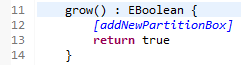
\includegraphics[width=0.4\textwidth]{eclipse_growDecl}
  \caption{Basic control flow to grow \texttt{box} \update}
  \label{fig:growDecl}
\end{center}
\end{figure}

\item[$\blacktriangleright$] Create and open the new pattern. You'll want it to match the invoking box with \emph{any} two partitions, so create a bound
\texttt{this} box, and free \texttt{firstPartitionInBox} and \texttt{lastPartitionInBox} partitions. You'll also need a variable set to create to represent the
new partition. The skeleton of your pattern should now resemble (Fig.~\ref{fig:growPattSkel}).

\vspace{0.5cm}

\begin{figure}[htbp]
\begin{center}
  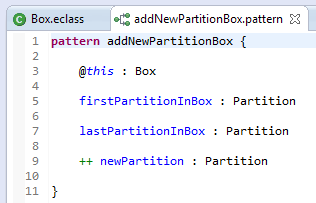
\includegraphics[width=0.5\textwidth]{eclipse_growPatternSkeleton}
  \caption{addPartitionsBox.pattern skeleton}
  \label{fig:growPattSkel}
\end{center}
\end{figure}

\item[$\blacktriangleright$] Next, we need to create an appropriate \emph{NAC} which will constrain the possible choices for \texttt{lastPartitionInBox}.
Create a \texttt{nextPartition} variable with an `!' operator (negation) preceding it immediately below \texttt{last\-Part\-it\-ion\-In\-Box}.

\vspace{0.5cm}

\item[$\blacktriangleright$] Now add \texttt{-> next : nextPartition} the the \texttt{lastPartition} scope. This
command will attempt to establish a \texttt{next} link from the last partition. Next, add \texttt{++ -> next: newPartition} (Fig.~\ref{fig:firstNAC}).
This line will only be reachable if the NAC fails! It establishes the \texttt{newPartition} as the final partition.

\begin{figure}[htbp]
\begin{center}
  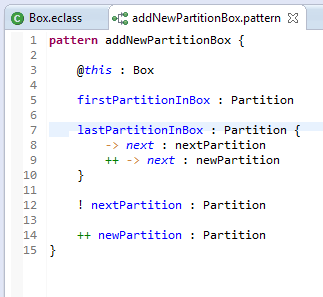
\includegraphics[width=0.5\textwidth]{eclipse_growLastNAC}
  \caption{Creating the first NAC \update}
  \label{fig:firstNAC}
\end{center}
\end{figure}

\vspace{0.5cm}

\item[$\blacktriangleright$] In a similar fashion, create a second NAC, \texttt{previousPartition}, for \texttt{firstPartitionInBox}. No new references have to
be created here, so all you need to establish is the link connecting \texttt{firstPartitionInBox} to the negative element, \texttt{previousPartition}
(Fig.~\ref{fig:growPatt}).

\begin{figure}[htp]
\begin{center}
  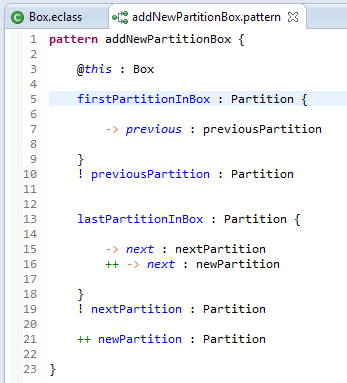
\includegraphics[width=0.55\textwidth]{eclipse_growFirstNAC}
  \caption{Pattern now with both NACs \update}
  \label{fig:growPatt}
\end{center}
\end{figure}

\item[$\blacktriangleright$] Now edit \texttt{@this} with appropriate links to the first and last partitions. Try using to auto-completion here for the
reference names!

\item[$\blacktriangleright$] The next step is to establish the \texttt{box} and \texttt{previous} references in our creation object variable,
\texttt{newPartition}. While you could write \texttt{++ -> box : this}, any link variables established here are set to `green,' and do not need to be explicitly
set with an \texttt{++} operator. This is because you cannot connect a `black' link to a `green' node. In other words, a positive object variable has a global
effect on all link variables declared in its scope.

\item[$\blacktriangleright$] Your pattern should now resemble Fig~\ref{fig:growAllLinks}. 

\begin{figure}[htp]
\begin{center}
  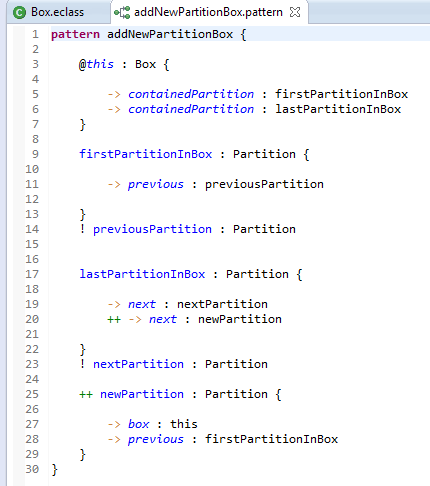
\includegraphics[width=0.65\textwidth]{eclipse_growLinks}
  \caption{A complete \emph{deterministic} pattern match \update}
  \label{fig:growAllLinks}
\end{center}
\end{figure}

\clearpage

\item[$\blacktriangleright$] We're not \emph{quite} done yet - our newest partition doesn't yet have a size. This means that not only do we need to make
another attribute contsraint, but \texttt{newPartition} needs to invoke a method in order to get the correct value. You can do this via a
\texttt{MethodCallExpression}, the structure of which is the similar to Java where:
\syntax{MethodCallExpression := (object\_variable\_expression | \\ parameter\_expression)`.'ID`('argument\_list `)'}


\item[$\blacktriangleright$] Your workspace should then resemble Fig.~\ref{fig:patternComplete}.

\begin{figure}[htp]
\begin{center}
  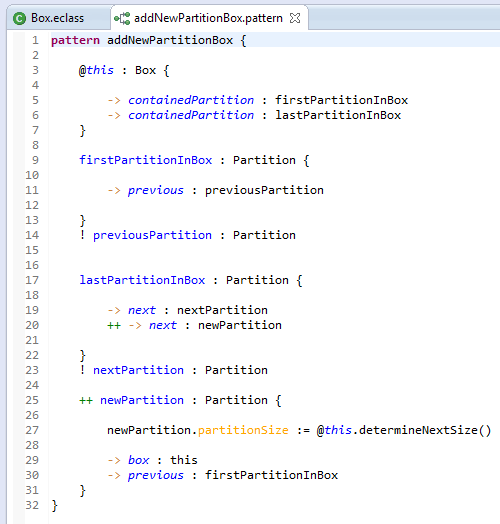
\includegraphics[width=0.9\textwidth]{eclipse_growFinished}
  \caption{Complete pattern for adding a new \texttt{partition} to \texttt{Box} \update}
  \label{fig:patternComplete}
\end{center}
\end{figure}

\vspace{0.5cm}

\item[$\blacktriangleright$] That's all! While NACs may be difficult to understand at first, as you can see, they're not hard to implement, and
can be used in a wide variety of applications. To see how this method is implemented in the visual syntax, check out Fig.~\ref{fig:growComplete} in the
previous section.

\end{itemize}